\Exercise
\label{Ex:interpolacio3}

En la competició FIFA 2023 que organitza Vicjove, l'avatar d'una jugadora del Lluçanès està llançant una falta a 20 metres de la porteria.  Un defensa de 2 metres es troba a mig camí entre el punt de llançament de la falta i la porteria. Si el seu xut té una velocitat inicial que ve donada pel vector $P'_0=(8,7)$, l'escaire és a una alçada de 3 metres i la velocitat d'entrada de la pilota a la porteria ve donada pel vector $P'_1=(5,0)$,  
\begin{enumerate}
  \item podrà superar el defensa?.
  \item Quina és l'alçada màxima que adquireix la pilota?
  \item Grafica tots els punts i una aproximació a la funció interpolada.
\end{enumerate}
NOTA important: La jugadora sospita que el rigor del programa FIFA pel que fa a la física pot ser més que dubtós, però afortunadament va aprovar Matemàtiques de primer de multimèdia i recorda que la interpolació d'Hermite segueix la fòrmula $Q_0(t)=T\cdot M \cdot G$ on
$  T= \begin{pmatrix}t^3 & t^2 & t & 1\end{pmatrix}$, 
$M= \begin{pmatrix}
              2 & -2 & 1 & 1 \\
              -3 & 3 & -2 & -1 \\
              0 & 0 & 1 & 0 \\
              1 & 0 & 0 & 0
        \end{pmatrix}$ i 
        $G= \begin{pmatrix}
              P_0 \\
              P_1 \\
              P'_0 \\
              P'_0
        \end{pmatrix}$

\Answer 

\begin{enumerate}
  \item podrà superar el defensa?.
  

  Comencem per graficar el problema:

\begin{center}
  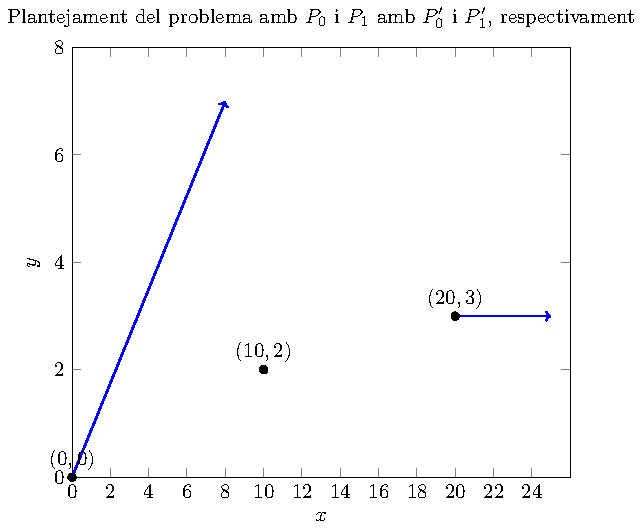
\includegraphics[width=5cm]{../figures/interpolaciohermite2inicial.pdf}
\end{center}

on es pot observar que $P_0=(0,0)$, $P_1=(20,3)$, $P'_0=(8,7)$ i $P'_1=(5,0)$.

{\em Nota}: és obvi que no es tracta d'un problema clàssic de tir parabòlic, ja que en aquest cas tindríem una velocitat horitzontal invariant. En el present exemple aquesta velocitat es redueix, la qual cosa implica una força contrària al moviment de la pilota amb component horitzontal (fricció del vent) que ha reduït aquesta component del valor inicial de 8 al final (en la posició de la porteria) de 5. De la mateixa manera, com que la component $Y$ de la velocitat és zero en arribar a la porteria, es podria deduir que la pilota just ha arribat al seu valor màxim. Més enllà d'això, obviarem la física del problema i ens centrarem en el problema d'interpolació plantejat (que, de fet, ens donarà una corba parametritzada de tercer grau i no de segon grau com seria esperat del problema físic).

La solució del problema es basa en parametritzar el polinomi que descriu el moviment. Segons la informació que ens donen sobre com descriure una interpolació cúbica d'Hermite, tenim:

\begin{eqnarray*}
  Q_0(t)&=&\begin{pmatrix}t^3 & t^2 & t & 1\end{pmatrix}
  \begin{pmatrix}
    2 & -2 & 1 & 1 \\
    -3 & 3 & -2 & -1 \\
    0 & 0 & 1 & 0 \\
    1 & 0 & 0 & 0
\end{pmatrix}
  \begin{pmatrix}
      P_0 \\
      P_1 \\
      P'_0 \\
      P'_1
  \end{pmatrix}\\
  \begin{pmatrix}
    x(t)&
    y(t)
  \end{pmatrix}&=&
  \begin{pmatrix}2t^3-3t^2+1 & -2t^3+3t^2&  t^3-2*t^2+t&t^3-t^2\end{pmatrix}
  \begin{pmatrix}
      0 &0 \\
      20 & 3\\
      8 & 7 \\
      5 & 0
  \end{pmatrix}\\
  \begin{pmatrix}
    x(t)&
    y(t)
  \end{pmatrix}&=&
  \begin{pmatrix}
    -27 t^3 +39 t^2 +8t&
    t^3-5t^2+7t
  \end{pmatrix}
\end{eqnarray*}

Aquesta interpolació es pot expressar com 

\[
\sigma(t)= (-27 t^3 +39 t^2 +8t) \uvec{i} +  (t^3-5t^2+7t)  \uvec{j}
\]

amb derivada

\[
\sigma'(t) = (-81t^2 + 78 t +8) \uvec{i} + (3t^2-10t+7) \uvec(j)  
\]

i és fàcil veure que es correspon amb les dades donades:

\begin{eqnarray*}
  P_0&=&\sigma(0) = 0 \uvec{i} + 0 \uvec{j}\\
  P_1&=&\sigma{1} = (-27+39+8) \uvec{i} + (1-5+7) \uvec{j} = 20 \uvec{i} + 3 \uvec{j}\\
  P'_0&=&\sigma(0) = 8 \uvec{i} + 7 \uvec{j}\\
  P'_1&=&\sigma'{1} = (-81+78+8) \uvec{i} + (3-10+7) \uvec{j} = 5 \uvec{i} + 0 \uvec{j}
\end{eqnarray*}

Per saber si supera el defensa, hem de veure quin valor de $y$ té la funció quan la $x=10$.

Això es pot aconseguir trobant el valor de $t$ per al qual $x=10$:
\[-27 t^3 +39 t^2 +8t=10\]
Solucionar una equació de tercer grau queda fora del coneixement d'aquest exercici, però podem mirar de trobar valors de $t$ que ens acotin el valor de $x$ i, d'aquesta manera, de $y$.

Per exemple, en primera aproximació, si $t=1/2$ tenim
\[-27 \left(\frac{1}{2}\right)^3 +39  \left(\frac{1}{2}\right)^2 +8\left(\frac{1}{2}\right)=-\frac{27}{8}+\frac{39}{4}+\frac{8}{2}=\frac{-27+78+32}{8}=\frac{83}{8}\approx 10\]

Per tant, $t=1/2$ sembla una bona aproximació inicial al temps que tarda la pilota en assolir $x=10$. En aquest valor, tenim:
\[
  y(t=1/2)=\left(\frac{1}{2}\right)^3-5\left(\frac{1}{2}\right)^2+7\frac{1}{2}=\frac{1}{8}-\frac{5}{4}+\frac{7}{2}=\frac{1-10+28}{8}=\frac{19}{8}>2
\]
NOTA: un simple càlcul amb matlab ens mostra que el $(x,y)=(10,2.34)$ quan $t=0.486$, o sigui que la primera aproximació feta és prou bona.

  \item Quina és l'alçada màxima que adquireix la pilota?

  Per trobar l'alçada màxima només cal mirar quan la primera derivada de la component y de la trajectòria es fa zero

  \[
    3t^2-10t+7=0\]
    que succeeix quan: 
    \[
      t=\frac{10 \pm \sqrt{100-4\cdot 3\cdot 7}}{6}\]
    és a dir, a $t_1=7/3$ i a $t=1$. El primer resultat queda exclços perquè és fora del rang de valors de $t$. El segon és el correcte i lliga amb la intuició inicial de que la pilota arribarà al seu màxim just quan toca el travesser. 

  \item Grafica tots els punts i una aproximació a la funció interpolada.
  
  el polinomi resultant serà

\begin{center}
  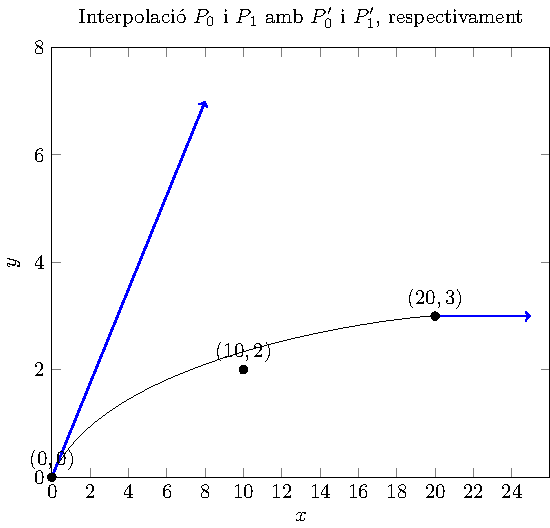
\includegraphics[width=5cm]{../figures/interpolaciohermite2final.pdf}
\end{center}
\end{enumerate}
